\chapter{Functional Requirements}\label{sec:Functional}

This chapter details the functional requirements of EFA, and in particular the
origin of each requirement as well as its priority and relevant test cases.

In the Ampersand system, each transformation which is done on the user
specification of their information system has a reasonable argument of
correctness. While a large part of ensuring this soundness falls to dynamic
testing, many components can be verified by static program analysis, e.g. by the
GHC typechecker and compiler. This requirement for EFA is the same as for
Ampersand - as much information as possible should be modelled by the Haskell
typechecker, which we assume to be sound. Therefore, typechecked programs are
also assumed to be correct with respect to those semantics which have been
encoded on the type level.
 
The Ampersand system also generates a large number and large variety of 
software design and requirements engineering artifacts, including 
documents in various markup formats, graphics and charts, and 
a prototype implementing the business logic encoding in the ADL file.
This large variety of functions must all work independently of 
each other, and in particular not interfere with each others' operation,
which is made very easy by the stateless nature of Haskell. However,
it is still possible to write Haskell code with very complex 
dependencies and code structure, making it very difficult to maintain,
upgrade and debug. EFA is required to be easy to maintain, and therefore
to integrate with the core Ampersand code base easily. 

 The functional requirements of Ampersand can therefore by summarized 
as correctness and modularity. 

\section{System Requirements}
%%-----------------------------SIDE EFFECTS---------------------------------%%
{\setlength{\tabcolsep}{6pt} %% Default is 6
    \begin{tabularx}{\textwidth}{>{\bfseries}m{3cm}X}
        Requirement & S1 \\ 
        \midrule
        \endhead
        Description  & Create pure functions with no unintended side effects
        \\	Rationale & The use of a functional programing languages requires 
        that this program be a pure function and does not have side effects, 
        however certain portions of the code requires the execution of side 
        effects to match the behaviour presented by external programs. In these 
        specific instances, the side effects are an intended behaviour.
        \\	Originator & Stakeholder/Developer
        
        \\ Test Case & Desired results can be confirmed as they will be 
        reflected in changes that take place in the Ampersand database.
        \\	Customer Satisfaction & 5 - Highest 
        \\	Priority & 5 - Highest 
        \vspace{12pt}
    \end{tabularx}
}

%%------------------ MODULES MUST FIT AMPERSAND FRAMEWORK-----------------%%

{\setlength{\tabcolsep}{6pt} %% Default is 6
    \begin{tabularx}{\textwidth}{>{\bfseries}m{3cm}X}
        Requirement & S2 \\ 
        \midrule
        \endhead
        Description  & Added modules must fit within Ampersand's current 
        framework
        \\	Rationale & Ampersand is a huge system that has weekly additions 
        to prevent conflict and breaking of existing packages/modules, an 
        effort should be made to minimize external dependencies. As EFA will be 
        an internal component of Ampersand, if a package that EFA depends on to 
        function properly is no longer maintained and breaks, it will in turn 
        break Ampersand.
        \\	Originator & Ampersand Creators (i.e. our client)        

        \\ Test case & Added modules are tested with cabal build inside of the
        Ampersand system as an internal component (i.e. System testing)
        \\	Customer Satisfaction & 4 - High 
        \\	Priority & 4 - High
        \vspace{12pt}
    \end{tabularx}
}
{\setlength{\tabcolsep}{6pt} %% Default is 6
    \begin{tabularx}{\textwidth}{>{\bfseries}m{3cm}X}
        Requirement & S3 \\ 
        \midrule
        \endhead
        Description  & All code must be maintainable. 
        \\	Rationale & For a system such as Ampersand to be maintainable, all 
        code for each of its components must be well documented so it may be 
        easily understood by those that were not a part of its original 
        development.
        \\	Originator & Ampersand Creators (i.e. our client)        
        
        \\ Test case & A literate program that produces a
        \edchange{WK}{latex}{\LaTeX{}} document. \edcomm{WK}{I do hope
          you still strive to pass this by adding the literate
          documents to the appendix!}
        \\	Customer Satisfaction & 4 - High 
        \\	Priority & 4 - High
        \vspace{12pt}
    \end{tabularx}
}

\section{Project Requirements}
%%--------------------------CORRECTNESS OF ECA TO SQL RULES ------------------%%
{\setlength{\tabcolsep}{6pt} %% Default is 6
    \begin{tabularx}{\textwidth}{>{\bfseries}C{3cm}X}
        Requirement & P1 \\ 
        \midrule
        \endhead
        Description  & Generated SQL queries must preserve the semantics of ECA 
        rules.  
        \\	Rationale & The translation would otherwise not be correct, as the 
        rules would be meaningless if their semantics are lost.
        \\	Originator & Ampersand Creators
        \\ Test Cases & Internal structure of ECA rules can be compared to SQL 
        queries through a series of datatype tests, each of which will result 
        in a traceable result or error message
        \\	Priority & 4 - High
        \vspace{12pt}
    \end{tabularx}
}

%%-------------------------TYPE CORRECTNESS ----------------------------------%%
{\setlength{\tabcolsep}{6pt} %% Default is 6
    \begin{tabularx}{\textwidth}{>{\bfseries}C{3cm}X}
        Requirement & P2 \\ 
        \midrule
        \endhead
        Description  & Provable Correctness: \edcomm{WK}{The use of
          dependent types in TypedSQL establishes some (safety)
          properties, but not the correctness proofs for the
          ECA-to-SQL conversion (see P1) that the Ampersand developers would be
          interested in. In its current form, this ``requirement''
          therefore looks quite confusing/confused.} Haskell like other functional 
        programming languages have 
        a strong type system which can be used for machine-checked proofs.
        \\	Rationale & Curry-Howard correspondence which states that the 
        return type of the function is analogous to a logical theorem, that is 
        subject to the hypothesis corresponding to the types of the argument 
        values that are passed to the function and thus the program used to 
        compute that function is analogous to a proof of that theorem.
        \\	Originator & Ampersand Creators
        \\ Test Cases & Using QuickCheck to test function properties.
        \\	Priority & 4 - High
        \vspace{12pt}
    \end{tabularx}
}

%\edcomm{YS}{Delete : Based on comment from WK, the requirement have been deleted}
%{\setlength{\tabcolsep}{6pt} %% Default is 6
%    \begin{tabularx}{\textwidth}{>{\bfseries}C{3cm}X}
%        Requirement & P3 \\ 
%        \midrule
%        \endhead
%        Description  & Generated SQL queries must be correctly implemented.
%        \edcomm{WK}{What do you mean by this? Would perhaps the
%          syntax- and type-correctness of the SQL statements coming
%          out of TypedSQL, and therewith the rationale of P1, be
%          appropriate here?}
%        \\	Rationale & Ampersand uses a MySQL database, for queries to be 
%        recognized and executed they must be error free. 
%        \\	Originator & Ampersand Creators
%        \\ Test Cases & Using MySQL WorkBench queries are manually executed and 
%        checked for errors.
%        \\	Priority & 4 - High
%        \vspace{12pt}
%    \end{tabularx}
%}


%%%%%%%%%%%%%%%%%%%%%%
%%% Non - Functional Requirements %%%%
%%%%%%%%%%%%%%%%%%%%%%

\chapter{Non-functional Requirements}\label{ch:NonFunc}

%\begin{figure}[!htb]
%	\centering
%	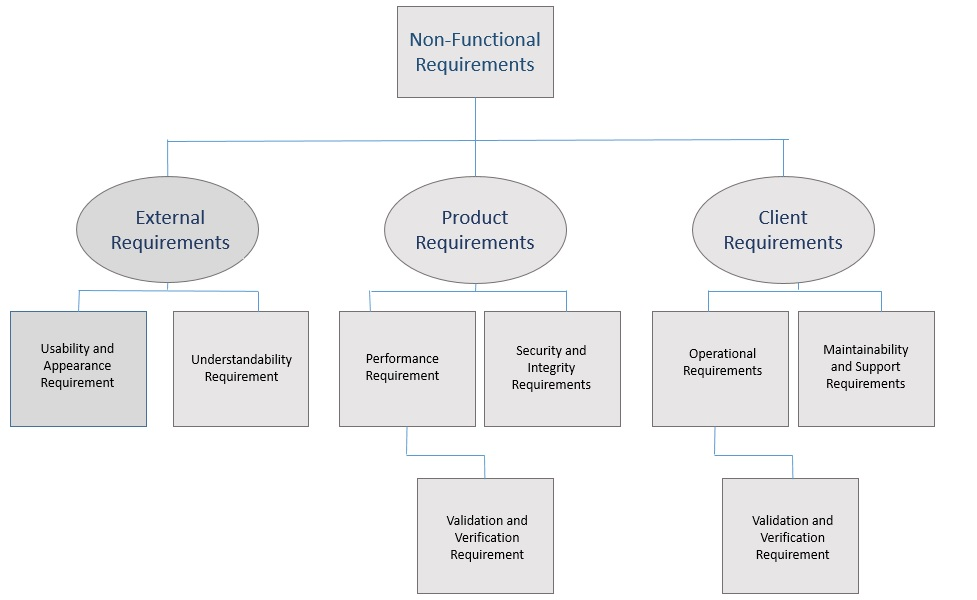
\includegraphics[width=0.8\textwidth]{../figures/NONFUNCTIONAL}
%	\caption{Tree of non-functional requirements as it relates to EFA}~\label{fig:figure2}
%\end{figure}

This chapter briefly describes the various non-functional requirements associated with the EFA project. 

\section{Look and Feel Requirements}\label{sec:LookAndFeel}
\begin{itemize}
    \item The product shall comply with Ampersand standards
    \item The product shall appear readable for Ampersand contributors
\end{itemize}

\section{Usability and Humanity Requirements}\label{sec:Usability}

\begin{itemize}
    \item \textit{Efficiency of use} 
        \begin{itemize}
           \item EFA is easy to use for any Ampersand user.
           \item The user can use EFA with accuracy, as they are provided with 
           the option to use EFA's automated service through the users 
           interface.
        \end{itemize}
    \item \textit{Ease of remembering}  
        \begin{itemize}
            \item EFA does not require the user to memorize protocols
        \end{itemize}
    \item \textit{Error rates} 
        \begin{itemize}
            \item EFA eliminates ECA rule violations caused by the user, 
            EFA's implementation is provably correct through Haskell 
            type-checking system.
        \end{itemize}
       
    \item \textit{Feedback} 
        \begin{itemize}
            \item User receive feed-back concerning the ECA rule 
            violations that have been resolved.
        \end{itemize}
    \item \textit{Overall satisfaction in using the product} 
    \begin{itemize}
        \item Users can be confident in using EFA as it is well tested and 
        provides accurate results which the user can confirm.
    \end{itemize}
\end{itemize}

\subsection{Personalization and Internationalization 
Requirements}\label{subsec:Personalization}
EFA is available only in English but can be adapted for other languages in 
later development versions.

\subsection{Learning Requirements}\label{subsec:LearningReq}
EFA has a shallow learning curve, more time is spent learning the Ampersand 
system. No training is necessary to use EFA as long as the user can operate 
Ampersand.

\section{Understandability and Politeness 
Requirements}\label{sec:Understandability}
Conceptually EFA is easy to understand and users will intuitively know what 
this product does for them. To further understandability, EFA feed back uses 
natural language that is familiar to the user and easy to understand. In 
addition, EFA hides all details of its construction from the user and provides 
the user. 

\ds{What are your understandability requirements for this project?}
\edcomm{JG}{kind of addressed}
\subsection{Accessibility Requirements}\label{Accessibility}
EFA is unable to individually confirm to disability requirements as it is an 
internal component of Ampersand.

\section{Performance Requirements}\label{sec:Performance}
\subsection{Speed and latency Requirements}\label{subsec:SpeedReq}
The use of EFA should not result in a noticeable time delay. EFA shall 
not take more than 3 seconds to complete in the worst case scenario.

\subsection{Safety-Critical Requirements}\label{subec:SafetyReq}
EFA will not expose sensitive information in the Ampersand system to outside 
sources or create new vulnerabilities.

\subsection{Precision or Accuracy Requirements}\label{subsec:AccuracyReq}
SQL queries generated by EFA is correct 100\% of the time with full coverage of 
all ECA rules that apply.
\edcomm{JG}{There's more to be added here, cant think of any right now}
 
\subsection{Reliability and Availability Requirements}\label{subsec:AvailReq}
EFA is available for use anytime Ampersand is used. In the event that Ampersand 
fails, then EFA will also be unavailable as it depends on Ampersand generated 
data taken from the user.

\subsection{Robustness or Fault-Tolerance Requirements}\label{subsec:FaultReq}

In the absence of ECA rule violations, EFA will continue to function and be on 
stand-by until a rule violation is triggered.

\subsection{Capacity Requirements}\label{subsec:CapacityReq}
Ampersand runs on individual machines; EFA as an internal component of 
Ampersand will be able to deal with any amount of data that Ampersand can 
handle. 

\subsection{Scalability and Extensibility 
Requirements}\label{subsec:ScalabilityReq}
EFA is capable of handling large volumes of data, and the translation of ECA 
rules to SQL queries requires a standard amount of time. The number of ECA 
rules is expected to expand as Ampersand etches closer to completion. 

%\subsection{Longevity Requirements}\label{subsec:LongevityReq}
%
%\edcomm{YS}{ECA rules can have interdependencies, these might be buried deep into the rules. Following a certain course of action under EFA, can trigger a deadlock situation where in the system is not able to come up with the best way to deal with inconsistencies in data. In the above example lets say the system is required to give a 2$ discount to the customer if the total cost(including) of his basket is greater than or equal to $10 and provide free shipping, but if the total cost (after discount ) is less than 10$ then 2$ needs to be added for shipping. This creates an infinite loop where the initial cost of the chair is a discount to $8 but then shipping is applied, and it becomes $10, which is again subjected to the discount. EFA needs to take care of such performance issue that would lead the system into a state if deadlock. EFA must have a run time capability to interrupt and send a message to the user about the existence of such conflicting requirements.
%}
%\edcomm{JG}{feel free to add that}
%%	I'm not too sure if the example is valid in our case, Does Ampersand automatically detect such conflicting requirements at an
%%	early stage? I've belive the existence of relational algebra can detect such conflicts, but what if they are introduced at run
%%	later, while the information system is in production?

%% Can you guys come up with a better example? The ones we've listed before don't really capture the performance of EFA

\section{Operational and Environmental Requirements}\label{sec:Operational}
\paragraph*{}
Any system that is currently running Ampersand will be able to run this product 
under a new verion and thus no new requirements have been introduced.
\ds{Either explicitly state the current requirements for running Ampersand, or
mention that any system currently running Ampersand will be able to run
the new version and thus no new requirements have been introduced}.

\section{Maintainability and Support Requirements}\label{sec:Support}
\paragraph*{}
All code submitted for this project must be maintainable, which mean it is well 
documented and comes with mathematical proof. EFA must make sure that each 
specification/error is traceable.
  
\ds{Pull out the explicit requirements and remove the fluff.}

\section{Security and Integrity Requirements}\label{sec:Security}
\paragraph*{}
 Access to the database and software which 
supports the various functions of Ampersand are run locally and subjected to the security system 
the user has in place on his or her work station.

\ds{The git repository is not the issue here, are there any security/integrity
	concerns for the data you will be handling or for the way your contribution
	will handle data?}
\ys{Removed information about git}
	
\section{Validation and Verification Requirements}\label{sec:Verification}
\paragraph*{}
\edcomm{YS}{Section needs to be re-written}

\section{Legal Requirements}\label{sec:Legal}
The implementation must eventually be included in Ampersand, which is licensed
under GPL3. To comply with this license, all of the implementation code must be
either written by us so we may license it under GPL, or must already be licensed
under GPL, or a compatible license, by its original author. We do not plan to
use existing code, other than as a reference.
